\documentclass[12pt, titlepage]{article}

\usepackage{fullpage}
\usepackage[round]{natbib}
\usepackage{multirow}
\usepackage{booktabs}
\usepackage{tabularx}
\usepackage{graphicx}
\usepackage{float}
\usepackage{hyperref}
\hypersetup{
    colorlinks,
    citecolor=black,
    filecolor=black,
    linkcolor=red,
    urlcolor=blue
}
\usepackage[round]{natbib}
\usepackage[dvipsnames]{xcolor}

\newcounter{acnum}
\newcommand{\actheacnum}{AC\theacnum}
\newcommand{\acref}[1]{AC\ref{#1}}

\newcounter{ucnum}
\newcommand{\uctheucnum}{UC\theucnum}
\newcommand{\uref}[1]{UC\ref{#1}}

\newcounter{mnum}
\newcommand{\mthemnum}{M\themnum}
\newcommand{\mref}[1]{M\ref{#1}}

\title{SE 3XA3: Module Guide\\Ratava}

\author{Team 9, Makiam Group
        \\ Aidan McPhelim - mcpheima
		\\ Alexie McDonald - mcdona16
		\\ Illya Pilipenko - pilipeni}

\date{\today}

%\input{../../Comments}

\begin{document}

\maketitle

\pagenumbering{roman}
\tableofcontents
\listoftables
\listoffigures

\begin{table}[bp]
\caption{\bf Revision History}
\begin{tabularx}{\textwidth}{p{4cm}p{2cm}X}
\toprule {\bf Date} & {\bf Version} & {\bf Notes}\\
\midrule
2018-09-18 & 0.0 & File structure added \\
2018-10-09 & 1.0 & Added sections 1, 2 and 6 \\
2018-10-09 & 1.1 & Module guide and Breakdown added\\
2018-10-09 & 1.2 & Uses hierarchy between modules added\\
2018-12-03 & 1.3 & Updated team name\\
2018-12-05 & 1.4 & Updated module decompositions\\
\bottomrule
\end{tabularx}
\end{table}

\newpage

\pagenumbering{arabic}

\section{Introduction}

Having separate modules within a software system makes things so much easier for said software's development, not only while making it, but long after the software has been deployed and people are going back to maintain it. Having this breakdown will also serve as a reference for new members beginning work on the software, so that they can gain an understanding of what the software is currently doing and save time.
\\\\
In this document you will find a breakdown of each module in the software, what it's purpose is and how it relates to the Requirement Specification Document(SRS). You will gain an understanding of why each module was made as it is, depending on things like fields that we want to be hidden because it is likely to change; a list of anticipated changes can be seen in section 2. The full module decomposition for this idea can be found in secion 5.



\section{Anticipated and Unlikely Changes} \label{SecChange}

This section lists possible changes to the system. According to the likeliness
of the change, the possible changes are classified into two
categories. Anticipated changes are listed in Section \ref{SecAchange}, and
unlikely changes are listed in Section \ref{SecUchange}.

\subsection{Anticipated Changes} \label{SecAchange}

Anticipated changes are the source of the information that is to be hidden
inside the modules. Ideally, changing one of the anticipated changes will only
require changing the one module that hides the associated decision. The approach
adapted here is called design for
change.

\begin{description}
\item[\refstepcounter{acnum} \actheacnum \label{acTemplate}:] The templates used to generate avatars.
\item[\refstepcounter{acnum} \actheacnum \label{acInput}:] The input criteria.
\item[\refstepcounter{acnum} \actheacnum \label{acFormat}:] The output file's format.
\item[\refstepcounter{acnum} \actheacnum \label{acHash}:] Available hash functions.
\item[\refstepcounter{acnum} \actheacnum \label{acColour}:] The range of colour pallets available to the user.
\item[\refstepcounter{acnum} \actheacnum \label{acOutputShape}:] The range of unique output shapes.
\item[\refstepcounter{acnum} \actheacnum \label{acInput}:] The graphics library used for generation.
\end{description}

\subsection{Unlikely Changes} \label{SecUchange}

The module design should be as general as possible. However, a general system is
more complex. Sometimes this complexity is not necessary. Fixing some design
decisions at the system architecture stage can simplify the software design. If
these decision should later need to be changed, then many parts of the design
will potentially need to be modified. Hence, it is not intended that these
decisions will be changed.

\begin{description}
\item[\refstepcounter{ucnum} \uctheucnum \label{ucIO}:] Input/Output devices
  (Input: File and/or Keyboard, Output: File, Memory, and/or Screen).
\item[\refstepcounter{ucnum} \uctheucnum \label{ucInput}:] The format in which the user enters the input String.
\item[\refstepcounter{ucnum} \uctheucnum \label{ucInput}:] The type of data the user enters as input.
\end{description}

\section{Module Hierarchy} \label{SecMH}

This section provides an overview of the module design. Modules are summarized
in a hierarchy decomposed by secrets in Table \ref{TblMH}. The modules listed
below, which are leaves in the hierarchy tree, are the modules that will
actually be implemented.

\begin{description}
\item [\refstepcounter{mnum} \mthemnum \label{mGH}:] Hash Generating Module
\item [\refstepcounter{mnum} \mthemnum \label{mGUI}:] GUI Module
\item [\refstepcounter{mnum} \mthemnum \label{mGD}:] Graphics Drawing Module
\item [\refstepcounter{mnum} \mthemnum \label{mTD}:] Template Drawing Module
\item [\refstepcounter{mnum} \mthemnum \label{mUH}:] Hash Using Module
\end{description}


\begin{table}[h!]
\centering
\begin{tabular}{p{0.3\textwidth} p{0.6\textwidth}}
\toprule
\textbf{Level 1} & \textbf{Level 2}\\
\midrule

{Hardware-Hiding Module} & ~ \\
\midrule

\multirow{7}{0.3\textwidth}{Behaviour-Hiding Module}
& GUI Module\\
& Graphics Drawing Module\\
& Hash Using Module\\
& Hash Generating Module\\
\midrule

\multirow{3}{0.3\textwidth}{Software Decision Module} & \\
& Template Drawing Module\\
\bottomrule

\end{tabular}
\caption{Module Hierarchy}
\label{TblMH}
\end{table}

\section{Connection Between Requirements and Design} \label{SecConnection}

The design of the system is intended to satisfy the requirements developed in
the SRS. In this stage, the system is decomposed into modules. The connection
between requirements and modules is listed in Table \ref{TblRT}.
\\\\
As can be seen in the SRS, the functional requirements in particular focus around a few specific concepts, like the hash functionality. In order to best satisfy these requirements, we decided it would be best to have a GenerateHash module, which handles all the types of Hash's available and does all related things within it. We decided to keep functionality which made use of the hash output separate since what we are generating and how we use that information is subject to change as can be seen in section 2.
\\\\
There are lots of requirements, non-functional and functional, which are about the users customization and usability, so we thought it would be best to keep all of that stuff in one neat module about the GUI, which can handle all user input and output.
\\\\
As for requirements regarding the generated avatar, we decided to split it into two modules, one for storing the templates so that it can be easily expanded, and one which handles the actual drawing and combining of these templates, which means if we want to change the way this is done, it is separate from the templates themselves.
\\\\
For a detailed view on how each individual requirement is represented by the modules, see section 6 for the Traceability Matrix.

\section{Module Decomposition} \label{SecMD}

Modules are decomposed according to the principle of ``information hiding''
proposed by \citet{ParnasEtAl1984}. The \emph{Secrets} field in a module
decomposition is a brief statement of the design decision hidden by the
module. The \emph{Services} field specifies \emph{what} the module will do
without documenting \emph{how} to do it. For each module, a suggestion for the
implementing software is given under the \emph{Implemented By} title. If the
entry is \emph{OS}, this means that the module is provided by the operating
system or by standard programming language libraries.  Also indicate if the
module will be implemented specifically for the software.

Only the leaf modules in the
hierarchy have to be implemented. If a dash (\emph{--}) is shown, this means
that the module is not a leaf and will not have to be implemented. Whether or
not this module is implemented depends on the programming language
selected.

\subsection{Hardware Hiding Modules (-)}

\begin{description}
\item[Secrets:]The data structure and algorithm used to implement the virtual
  hardware.
\item[Services:]Serves as a virtual hardware used by the rest of the
  system. This module provides the interface between the hardware and the
  software. So, the system can use it to display outputs or to accept inputs.
\item[Implemented By:] OS
\end{description}

\subsection{Behaviour-Hiding Module}

\begin{description}
\item[Secrets:]The contents of the required behaviours.
\item[Services:]Includes programs that provide externally visible behaviour of
  the system as specified in the software requirements specification (SRS)
  documents. This module serves as a communication layer between the
  hardware-hiding module and the software decision module. The programs in this
  module will need to change if there are changes in the SRS.
\item[Implemented By:] --
\end{description}

\subsubsection{Hash Generating Module (\mref{mGH})}

\begin{description}
\item[Secrets:]Generates a hash value.
\item[Services:] Generates a hash value from a given string using a chosen hashing function.
\item[Implemented By:] Using hashlib to generate a hash value from a string.
\end{description}

\subsubsection{GUI Module (\mref{mGUI})}

\begin{description}
\item[Secrets:]Allows user to interface with system.
\item[Services:]\textcolor{red}{ Lets the user pick the avatar template, The colours used, the file information, and what string to use for hashing with what kind of hashing function.}
\item[Implemented By:] Using tkinter to create a visual interface for the user.
\end{description}

\subsubsection{Graphics Drawing Module (\mref{mGD})}

\begin{description}
\item[Secrets:] Creates avatar image file.
\item[Services:] Creates the .jpg file with the generated avatar at the user-specified location, and opens it.
\item[Implemented By:] Using \mref{mUH}, \mref{mTD}, and \mref{mGUI} to get information on what to make the avatar look like, and Pillow to create the image file.
\end{description}

\subsubsection{Hash Using Module (\mref{mUH})}

\begin{description}
\item[Secrets:]Uses a hash value to randomize avatar generation.
\item[Services:]Takes a hash value and uses it to generate sets of colours and randomize certain avatar parts.
\item[Implemented By:] Converting parts of a hash value to integers within the part tuple size, and converting parts of a hash value to integers between 0-255 for RGB values.
\end{description}

\subsection{Software Decision Module}

\begin{description}
\item[Secrets:] The design decision based on mathematical theorems, physical
  facts, or programming considerations. The secrets of this module are
  \emph{not} described in the SRS.
\item[Services:] Includes data structure and algorithms used in the system that
  do not provide direct interaction with the user.
  % Changes in these modules are more likely to be motivated by a desire to
  % improve performance than by externally imposed changes.
\item[Implemented By:] --
\end{description}

\subsubsection{Template Drawing Module (\mref{mTD})}

\begin{description}
\item[Secrets:]Provides avatar templates.
\item[Services:]\textcolor{red}{Provides information on what avatar templates there are and how to draw each template.}
\item[Implemented By:]\textcolor{red}{List of available templates, and their corresponding pixel arrays.}
\end{description}


\section{Traceability Matrix} \label{SecTM}

This section shows two traceability matrices: between the modules and the
requirements and between the modules and the anticipated changes.

% the table should use mref, the requirements should be named, use something
% like fref
\begin{table}[H]
\centering
\begin{tabular}{| c | c | c | c | c | c |}
\toprule
\textbf{Req.} & \textbf{Module 1} & \textbf{Module 2} & \textbf{Module 3} & \textbf{Module 4} & \textbf{Module 5}\\
\hline
R1 &  & X &  &  &  \\
R2 &  &  &  &  & X \\
R3 &  & X &  &  &  \\
R4 &  & X &  &  &  \\
R5 &  & X &  &  &  \\
R6 &  & X &  &  & X \\
R7 &  & X &  &  &  \\
R8 &  & X &  &  &  \\
R9 &  & X &  &  &  \\
R10 &  & X &  &  &  \\
R11 &  & X &  &  &  \\
R12 &  & X &  &  &  \\
R13 &  & X &  &  &  \\
R14 &  & X &  &  &  \\
R15 &  & X &  &  &  \\
R16 &  & X &  &  &  \\
R17 &  & X &  &  &  \\
R18 & X &  & X & X & X \\
R19 & X &  & X & X & X \\
R20 & &  & X & X & \\
R21 &  &  &  &  &  \\
R22 &  &  &  &  &  \\
R23 &  &  &  &  &  \\
R24 &  &  &  &  &  \\
R25 &  &  &  &  &  \\
R26 &  &  &  & X &  \\
R27 & X &  &  &  &  \\
R28 &  &  & X &  &  \\
R29 & X & X & X & X & X \\
R30 &  &  &  &  &  \\
R31 & X &  &  &  & X \\
R32 & X &  &  &  &  \\
R33 &  &  &  &  &  \\
R34 &  &  & X & X &  \\
R35 &  &  &  &  &  \\
R36 &  &  &  &  &  \\
\bottomrule
\end{tabular}
\caption{Trace Between Requirements and Modules}
\label{TblRT}
\end{table}

\begin{table}[H]
\centering
\begin{tabular}{| c | c | c | c | c | c |}
\toprule
\textbf{AC} & \textbf{Module 1} & \textbf{Module 2} & \textbf{Module 3} & \textbf{Module 4} & \textbf{Module 5}\\
\toprule
AC1 &  &  &  & X &  \\
AC2 &  & X &  &  &  \\
AC3 &  & X &  &  &  \\
AC4 & X &  &  &  &  \\
AC5 &  & X &  &  &  \\
AC6 &  &  & X &  &  \\
AC7 &  &  & X &  &  \\
\bottomrule
\end{tabular}
\caption{Trace Between Anticipated Changes and Modules}
\label{TblACT}
\end{table}

\section{Use Hierarchy Between Modules} \label{SecUse}

In this section, the uses hierarchy between modules is
provided. \citet{Parnas1978} said of two programs A and B that A {\em uses} B if
correct execution of B may be necessary for A to complete the task described in
its specification. That is, A {\em uses} B if there exist situations in which
the correct functioning of A depends upon the availability of a correct
implementation of B.  Figure \ref{FigUH} illustrates the use relation between
the modules. It can be seen that the graph is a directed acyclic graph
(DAG). Each level of the hierarchy offers a testable and usable subset of the
system, and modules in the higher level of the hierarchy are essentially simpler
because they use modules from the lower levels.

\begin{figure}[H]
\centering
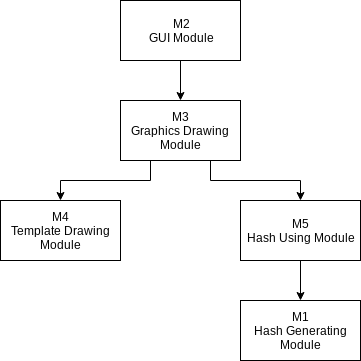
\includegraphics[width=0.7\textwidth]{UsesHierarchy.png}
\caption{Use hierarchy among modules}
\label{FigUH}
\end{figure}

%\section*{References}

\bibliographystyle {plainnat}
\bibliography {MG}

\end{document}
